% Options for packages loaded elsewhere
\PassOptionsToPackage{unicode}{hyperref}
\PassOptionsToPackage{hyphens}{url}
%
\documentclass[
]{article}
\usepackage{lmodern}
\usepackage{amssymb,amsmath}
\usepackage{ifxetex,ifluatex}
\ifnum 0\ifxetex 1\fi\ifluatex 1\fi=0 % if pdftex
  \usepackage[T1]{fontenc}
  \usepackage[utf8]{inputenc}
  \usepackage{textcomp} % provide euro and other symbols
\else % if luatex or xetex
  \usepackage{unicode-math}
  \defaultfontfeatures{Scale=MatchLowercase}
  \defaultfontfeatures[\rmfamily]{Ligatures=TeX,Scale=1}
\fi
% Use upquote if available, for straight quotes in verbatim environments
\IfFileExists{upquote.sty}{\usepackage{upquote}}{}
\IfFileExists{microtype.sty}{% use microtype if available
  \usepackage[]{microtype}
  \UseMicrotypeSet[protrusion]{basicmath} % disable protrusion for tt fonts
}{}
\makeatletter
\@ifundefined{KOMAClassName}{% if non-KOMA class
  \IfFileExists{parskip.sty}{%
    \usepackage{parskip}
  }{% else
    \setlength{\parindent}{0pt}
    \setlength{\parskip}{6pt plus 2pt minus 1pt}}
}{% if KOMA class
  \KOMAoptions{parskip=half}}
\makeatother
\usepackage{xcolor}
\IfFileExists{xurl.sty}{\usepackage{xurl}}{} % add URL line breaks if available
\IfFileExists{bookmark.sty}{\usepackage{bookmark}}{\usepackage{hyperref}}
\hypersetup{
  pdftitle={My very first post and how I created this website},
  pdfauthor={Karen Chu Sam},
  hidelinks,
  pdfcreator={LaTeX via pandoc}}
\urlstyle{same} % disable monospaced font for URLs
\usepackage[margin=1in]{geometry}
\usepackage{color}
\usepackage{fancyvrb}
\newcommand{\VerbBar}{|}
\newcommand{\VERB}{\Verb[commandchars=\\\{\}]}
\DefineVerbatimEnvironment{Highlighting}{Verbatim}{commandchars=\\\{\}}
% Add ',fontsize=\small' for more characters per line
\usepackage{framed}
\definecolor{shadecolor}{RGB}{248,248,248}
\newenvironment{Shaded}{\begin{snugshade}}{\end{snugshade}}
\newcommand{\AlertTok}[1]{\textcolor[rgb]{0.94,0.16,0.16}{#1}}
\newcommand{\AnnotationTok}[1]{\textcolor[rgb]{0.56,0.35,0.01}{\textbf{\textit{#1}}}}
\newcommand{\AttributeTok}[1]{\textcolor[rgb]{0.77,0.63,0.00}{#1}}
\newcommand{\BaseNTok}[1]{\textcolor[rgb]{0.00,0.00,0.81}{#1}}
\newcommand{\BuiltInTok}[1]{#1}
\newcommand{\CharTok}[1]{\textcolor[rgb]{0.31,0.60,0.02}{#1}}
\newcommand{\CommentTok}[1]{\textcolor[rgb]{0.56,0.35,0.01}{\textit{#1}}}
\newcommand{\CommentVarTok}[1]{\textcolor[rgb]{0.56,0.35,0.01}{\textbf{\textit{#1}}}}
\newcommand{\ConstantTok}[1]{\textcolor[rgb]{0.00,0.00,0.00}{#1}}
\newcommand{\ControlFlowTok}[1]{\textcolor[rgb]{0.13,0.29,0.53}{\textbf{#1}}}
\newcommand{\DataTypeTok}[1]{\textcolor[rgb]{0.13,0.29,0.53}{#1}}
\newcommand{\DecValTok}[1]{\textcolor[rgb]{0.00,0.00,0.81}{#1}}
\newcommand{\DocumentationTok}[1]{\textcolor[rgb]{0.56,0.35,0.01}{\textbf{\textit{#1}}}}
\newcommand{\ErrorTok}[1]{\textcolor[rgb]{0.64,0.00,0.00}{\textbf{#1}}}
\newcommand{\ExtensionTok}[1]{#1}
\newcommand{\FloatTok}[1]{\textcolor[rgb]{0.00,0.00,0.81}{#1}}
\newcommand{\FunctionTok}[1]{\textcolor[rgb]{0.00,0.00,0.00}{#1}}
\newcommand{\ImportTok}[1]{#1}
\newcommand{\InformationTok}[1]{\textcolor[rgb]{0.56,0.35,0.01}{\textbf{\textit{#1}}}}
\newcommand{\KeywordTok}[1]{\textcolor[rgb]{0.13,0.29,0.53}{\textbf{#1}}}
\newcommand{\NormalTok}[1]{#1}
\newcommand{\OperatorTok}[1]{\textcolor[rgb]{0.81,0.36,0.00}{\textbf{#1}}}
\newcommand{\OtherTok}[1]{\textcolor[rgb]{0.56,0.35,0.01}{#1}}
\newcommand{\PreprocessorTok}[1]{\textcolor[rgb]{0.56,0.35,0.01}{\textit{#1}}}
\newcommand{\RegionMarkerTok}[1]{#1}
\newcommand{\SpecialCharTok}[1]{\textcolor[rgb]{0.00,0.00,0.00}{#1}}
\newcommand{\SpecialStringTok}[1]{\textcolor[rgb]{0.31,0.60,0.02}{#1}}
\newcommand{\StringTok}[1]{\textcolor[rgb]{0.31,0.60,0.02}{#1}}
\newcommand{\VariableTok}[1]{\textcolor[rgb]{0.00,0.00,0.00}{#1}}
\newcommand{\VerbatimStringTok}[1]{\textcolor[rgb]{0.31,0.60,0.02}{#1}}
\newcommand{\WarningTok}[1]{\textcolor[rgb]{0.56,0.35,0.01}{\textbf{\textit{#1}}}}
\usepackage{graphicx,grffile}
\makeatletter
\def\maxwidth{\ifdim\Gin@nat@width>\linewidth\linewidth\else\Gin@nat@width\fi}
\def\maxheight{\ifdim\Gin@nat@height>\textheight\textheight\else\Gin@nat@height\fi}
\makeatother
% Scale images if necessary, so that they will not overflow the page
% margins by default, and it is still possible to overwrite the defaults
% using explicit options in \includegraphics[width, height, ...]{}
\setkeys{Gin}{width=\maxwidth,height=\maxheight,keepaspectratio}
% Set default figure placement to htbp
\makeatletter
\def\fps@figure{htbp}
\makeatother
\setlength{\emergencystretch}{3em} % prevent overfull lines
\providecommand{\tightlist}{%
  \setlength{\itemsep}{0pt}\setlength{\parskip}{0pt}}
\setcounter{secnumdepth}{-\maxdimen} % remove section numbering

\title{My very first post and how I created this website}
\author{Karen Chu Sam}
\date{2020-02-17T21:13:14-05:00}

\begin{document}
\maketitle

\hypertarget{r-markdown}{%
\section{R Markdown}\label{r-markdown}}

I am very excited to be writing my very first post of this blog. So, let
me start by telling you how I created this very nice minimalist website
in R.

I first started learning R in my stats class at university and I thought
that R was only a programming language for statistical analysis. Little
I knew about the power of R\ldots{} As it so happens, for a course
project, my teammate and I would copy the code chunks, the output and
the graphs from R, and then paste them in LaTex. It was a very
time-consuming process that got us more focused in the correct code for
LaTex than in the analysis itself.

Just recently, while taking the \emph{Data Scientist's Toolbox} in the
\emph{Data Science} course from Coursera, I learned about the existence
of R markdown and how useful it could be for small projects and even
simple websites such as this. I thought I could give it a chance and try
it out.

So what is R markdown?

R markdown is markdown language created for R, so that text and R code
could be integrated in the same document. By doing this, you can be sure
that the R code written in the document is working fine.

How did I create the website with R markdown?

To create a webiste with R markdown you need the blogdown package which
uses R markdown to create websites. For this website, I used R studio
and went to File -\textgreater{} New Project -\textgreater{} New
Directory -\textgreater{} Website using blogdown. It opens a window
where you choose options for your website and a Hugo theme. Hugo is a
static site generator and is the default site generator in blogdown. To
choose a theme, go to \url{https://gohugo.io/} and select the theme you
like. Finally, click on create! What happends then is that R is
installing the blogdown package, blogdown downloads the theme you chose
in Hugo. Templates in Hugo would normally include the following files: *
config.toml * public * content * static * themes I created my github
account where I push and commit. use \url{https://www.netlify.com} to
deploy the website. this is the default site generator in blogdown which
a static site generator. I pushed and committed all the files in the
workspace to github and then deploy the website in netlify.

Now, everytime I create a new post, I go to the post file of my
workspace and write a file in R markdown.

You can embed an R code chunk like this:

\begin{Shaded}
\begin{Highlighting}[]
\KeywordTok{summary}\NormalTok{(cars)}
\CommentTok{##      speed           dist       }
\CommentTok{##  Min.   : 4.0   Min.   :  2.00  }
\CommentTok{##  1st Qu.:12.0   1st Qu.: 26.00  }
\CommentTok{##  Median :15.0   Median : 36.00  }
\CommentTok{##  Mean   :15.4   Mean   : 42.98  }
\CommentTok{##  3rd Qu.:19.0   3rd Qu.: 56.00  }
\CommentTok{##  Max.   :25.0   Max.   :120.00}
\NormalTok{fit <-}\StringTok{ }\KeywordTok{lm}\NormalTok{(dist }\OperatorTok{~}\StringTok{ }\NormalTok{speed, }\DataTypeTok{data =}\NormalTok{ cars)}
\NormalTok{fit}
\CommentTok{## }
\CommentTok{## Call:}
\CommentTok{## lm(formula = dist ~ speed, data = cars)}
\CommentTok{## }
\CommentTok{## Coefficients:}
\CommentTok{## (Intercept)        speed  }
\CommentTok{##     -17.579        3.932}
\end{Highlighting}
\end{Shaded}

\hypertarget{including-plots}{%
\section{Including Plots}\label{including-plots}}

You can also embed plots. See Figure @ref(fig:pie) for example:

\begin{Shaded}
\begin{Highlighting}[]
\KeywordTok{par}\NormalTok{(}\DataTypeTok{mar =} \KeywordTok{c}\NormalTok{(}\DecValTok{0}\NormalTok{, }\DecValTok{1}\NormalTok{, }\DecValTok{0}\NormalTok{, }\DecValTok{1}\NormalTok{))}
\KeywordTok{pie}\NormalTok{(}
  \KeywordTok{c}\NormalTok{(}\DecValTok{280}\NormalTok{, }\DecValTok{60}\NormalTok{, }\DecValTok{20}\NormalTok{),}
  \KeywordTok{c}\NormalTok{(}\StringTok{'Sky'}\NormalTok{, }\StringTok{'Sunny side of pyramid'}\NormalTok{, }\StringTok{'Shady side of pyramid'}\NormalTok{),}
  \DataTypeTok{col =} \KeywordTok{c}\NormalTok{(}\StringTok{'#0292D8'}\NormalTok{, }\StringTok{'#F7EA39'}\NormalTok{, }\StringTok{'#C4B632'}\NormalTok{),}
  \DataTypeTok{init.angle =} \DecValTok{-50}\NormalTok{, }\DataTypeTok{border =} \OtherTok{NA}
\NormalTok{)}
\end{Highlighting}
\end{Shaded}

\begin{figure}
\centering
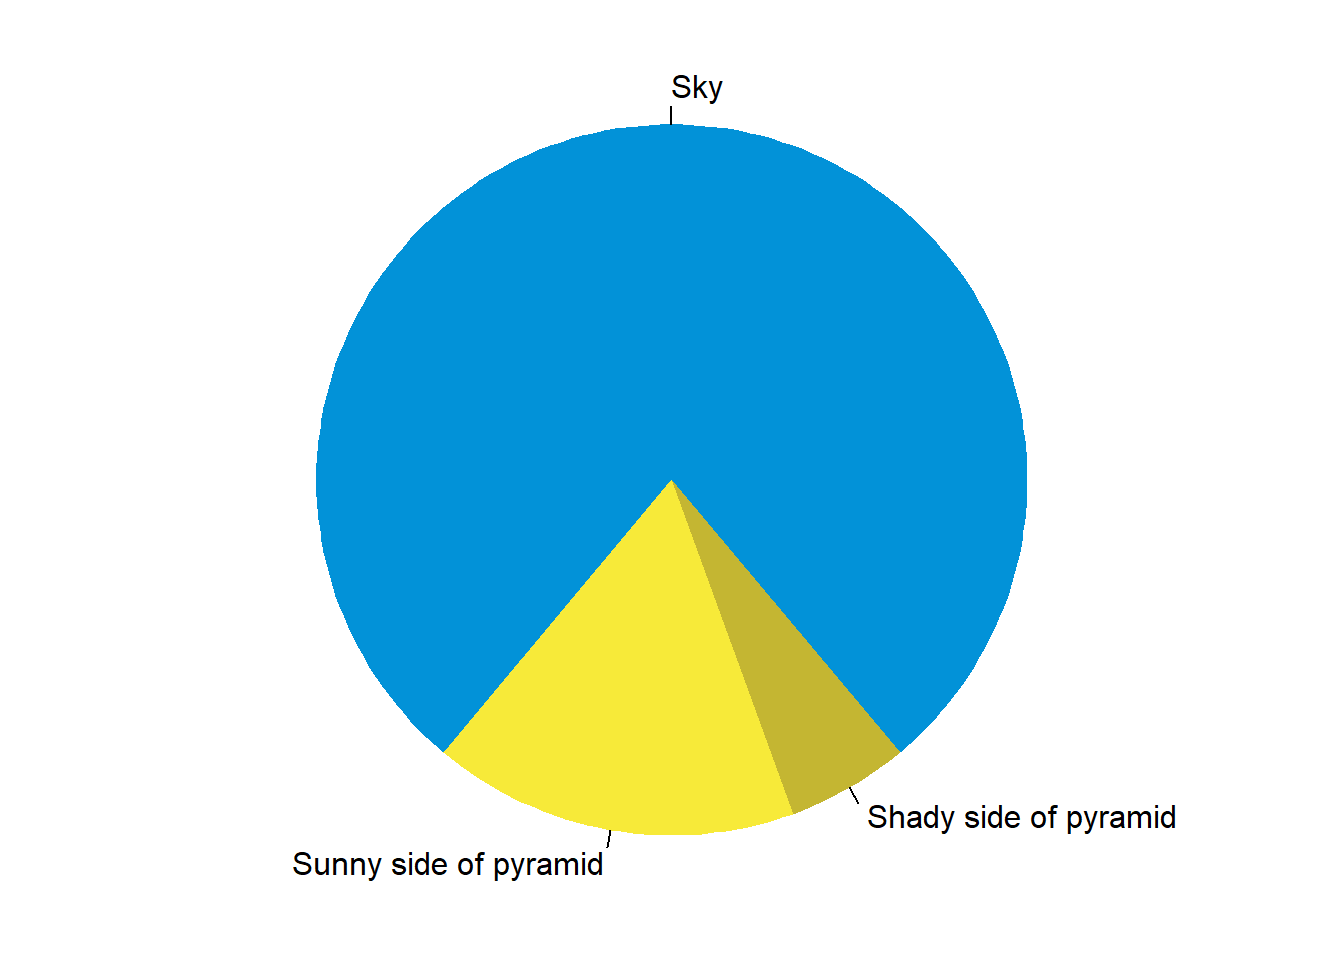
\includegraphics{2015-07-23-r-rmarkdown_files/figure-latex/pie-1.pdf}
\caption{A fancy pie chart.}
\end{figure}

\end{document}
